% !TEX program = xelatex
% IA712 - Projet B : Recherche et sauvetage autonome - publication 2 pages, style IEEE (FR)
\documentclass[10pt,twocolumn,a4paper]{article}

\usepackage{fontspec}
\usepackage{amsmath}
\usepackage[a4paper,margin=1.5cm]{geometry}
\usepackage{graphicx}
\graphicspath{{img/}}
\usepackage{xcolor}
\usepackage{tikz}
\usetikzlibrary{arrows.meta,positioning,shapes.geometric,fit,backgrounds,calc,decorations.pathreplacing}
\usepackage{booktabs}
\usepackage{caption}
\captionsetup{font=footnotesize,labelfont=bf,skip=2pt}
\usepackage{subcaption}
\usepackage{titlesec}
\titlespacing*{\section}{0pt}{5pt}{2pt}
\titleformat{\section}{\normalfont\large\bfseries\color{nccblue}}{\thesection}{0.5em}{}
\usepackage[french]{babel}
\usepackage[colorlinks=true,linkcolor=nccblue,citecolor=nccblue,urlcolor=nccblue]{hyperref}

% -- couleurs du theme --
\definecolor{nccblue}{HTML}{1F4E79}
\definecolor{nccsky}{HTML}{1F6FEB}
\definecolor{nccorange}{HTML}{FB8500}
\definecolor{nccgreen}{HTML}{2DA44E}
\definecolor{nccred}{HTML}{D1242F}
\definecolor{nccgray}{HTML}{EEF1F5}
\definecolor{nccdark}{HTML}{222831}

% -- styles tikz --
\tikzset{
  box/.style={rounded corners=2pt,draw=nccblue,fill=nccgray,align=center,inner sep=2pt,font=\tiny,minimum height=5mm,text width=16mm},
  proc/.style={box,fill=white},
  phase1/.style={box,fill=nccsky!15,draw=nccsky},
  phase2/.style={box,fill=nccorange!15,draw=nccorange},
  btnode/.style={box,fill=nccblue!12,draw=nccblue},
  io/.style={box,fill=nccgreen!12,draw=nccgreen,rounded corners=5pt},
  ar/.style={-{Latex[length=1.6mm]},draw=nccdark!70,semithick},
  arl/.style={ar,font=\tiny,inner sep=1pt},
}

\newcommand{\head}[1]{\par\smallskip\noindent\textbf{\color{nccblue}#1}\ \ignorespaces}

\setlength{\textfloatsep}{6pt plus 2pt minus 2pt}
\setlength{\floatsep}{6pt plus 2pt minus 2pt}
\setlength{\intextsep}{6pt plus 2pt minus 2pt}

\begin{document}
\sloppy

% BLOC TITRE
\twocolumn[
\begin{@twocolumnfalse}
\begin{center}
  {\LARGE\bfseries\color{nccblue} Recherche et sauvetage autonome avec un seul TurtleBot~4 :\par}
  \vspace{2pt}
  {\LARGE\bfseries\color{nccblue} une mission en deux phases orchestr\'ee par un arbre de comportement\par}
  \vspace{6pt}
  {\normalsize\bfseries Équipe RobotZ\par}\smallskip
  {\large Julien GIMENEZ \quad Hugo FANCHINI \quad Paul CINTRA \quad Yimou ZHANG\par}
  \vspace{3pt}
  {\footnotesize \texttt{\{julien.gimenez, hugo.fanchini, paul.cintra, yimou.zhang\}@telecom-paris.fr}\par}
  \vspace{2pt}
  {\footnotesize Projet B - IA712 Robotique mobile, projet final - T\'el\'ecom Paris\par}
  \vspace{2pt}
  {\footnotesize D\'ep\^ot : \url{https://github.com/YiZeems/autonomous-search-and-rescue}\par}
\end{center}
\vspace{4pt}
\noindent\fcolorbox{nccblue}{nccblue!6}{\parbox{\dimexpr\linewidth-2\fboxsep-2\fboxrule}{%
\small\textbf{R\'esum\'e-}Un unique TurtleBot~4 explore de mani\`ere autonome une ar\`ene de catastrophe
inconnue et cloisonn\'ee, construit une carte par SLAM et localise quatre « victimes » (AprilTags) en
projetant les d\'etections de la cam\'era dans le rep\`ere global \texttt{map} avec \texttt{tf2}. La
d\'ecision est confi\'ee \`a un \emph{arbre de comportement} (et non \`a une machine \`a \'etats finis,
comme l'exige le sujet~[1]) qui orchestre une \textbf{mission en deux phases} : d'abord l'exploration par
fronti\`eres, puis une inspection des pi\`eces d\'eriv\'ee de la carte. Nous montrons que l'exploration
pure ach\`eve la carte mais manque structurellement les victimes, car la cam\'era n'approche jamais assez
pr\`es des tags muraux ; une seconde phase autonome, qui d\'erive une pose d'inspection par pi\`ece
d\'ecouverte, comble cet \'ecart. L'ex\'ecution finale autonome en un clic atteint \textbf{97,35\,\% de
couverture et 4/4 victimes}. Cet article pr\'esente l'architecture, la th\'eorie sous-jacente et une
\'evaluation quantitative.}}
\vspace{8pt}
\end{@twocolumnfalse}
]

% 1. INTRODUCTION
\section{Introduction}
La robotique de recherche et sauvetage vise \`a envoyer des machines autonomes dans des zones de
catastrophe o\`u l'humain ne peut p\'en\'etrer sans risque. Le sc\'enario « Projet~B » d'IA712~[1]
formalise cela comme un probl\`eme concret : un robot mobile est d\'epos\'e dans un b\^atiment simul\'e et
cloisonn\'e qu'il ne conna\^it pas \emph{a priori}, et doit \emph{explorer de fa\c{c}on autonome},
construire une carte coh\'erente, \emph{localiser les victimes} repr\'esent\'ees par des marqueurs
visuels, et \emph{reporter leurs coordonn\'ees} dans un rep\`ere global fixe - le tout sans intervention
humaine. Le sujet impose plusieurs contraintes strictes : l'exploration doit \^etre autonome (fronti\`eres
ou RRT), la carte doit couvrir plus de 90\,\% de la surface et \^etre annot\'ee de chaque victime, les
positions doivent \^etre projet\'ees dans le rep\`ere \texttt{map}, la cha\^ine doit se lancer en \emph{un
clic}, et surtout la d\'ecision doit \^etre un arbre de comportement plut\^ot qu'une machine \`a \'etats
finis.

Notre plateforme est un TurtleBot~4 (base Create~3, RPLIDAR~A1M8, cam\'era OAK-D) simul\'e sous Ignition
Gazebo Fortress et ROS\,2 Humble. L'ar\`ene \texttt{rescue\_arena} est un b\^atiment de quatre pi\`eces
portant un AprilTag « victime » sur un mur ext\'erieur de chacune. \`A partir d'un unique lancement, le
robot cartographie le b\^atiment par SLAM, visite chaque pi\`ece, d\'etecte les quatre tags, les projette
dans le rep\`ere \texttt{map} et s'arr\^ete sur une carte annot\'ee propre. L'id\'ee centrale de ce
travail est que la compl\'etude de la carte et la couverture des victimes sont des objectifs
\emph{distincts} : un robot peut cartographier parfaitement une pi\`ece depuis sa porte sans jamais
approcher sa cam\'era du tag mural. Nous d\'ecoupons donc la mission en deux phases autonomes
coordonn\'ees par un arbre de comportement, ce que nous \'evaluons ci-dessous.

% 2. SYSTEME
\section{Syst\`eme et m\'ethode}
\head{Architecture.} L'espace de travail est divis\'e en quatre paquets ROS\,2 pour permettre le travail
en parall\`ele : \texttt{rescue\_bringup} (lancement en un clic et configurations Nav2/SLAM/AprilTag),
\texttt{rescue\_robot} (un « m\'egapaquet » Python regroupant exploration, perception, inspection et
r\'esultats), \texttt{rescue\_world} (l'ar\`ene Ignition et les cibles AprilTag en voxels, source unique
de v\'erit\'e pour le placement des victimes), et \texttt{rescue\_decision} (l'ex\'ecuteur C++
\texttt{BehaviorTree.CPP\,v3}). La Fig.~\ref{fig:arch} montre le flux de topics. L'arbre de comportement
est l'\emph{orchestrateur} : il active l'explorateur de Phase~1 et l'inspecteur de Phase~2 via les topics
\texttt{/mission/*}, tandis que les n\oe uds Python font le travail. Le SLAM alimente en continu la carte
vers l'exploration, la couverture, Nav2 et l'inspection.

\begin{figure}[t]
\centering
\resizebox{\linewidth}{!}{%
\begin{tikzpicture}[node distance=4.5mm and 7mm]
  \node[io] (robot) {TurtleBot~4\\\scriptsize Create~3 + RPLIDAR + OAK-D};
  \node[proc,below=10mm of robot] (slam) {\textbf{slam\_toolbox}\\\scriptsize async + fermeture de boucle};
  \node[proc,right=of slam] (metric) {\textbf{coverage\_}\\\textbf{evaluator}};
  \node[proc,above=of metric] (april) {\textbf{apriltag\_ros}\\\scriptsize tag36h11};
  \node[btnode,right=14mm of metric,text width=30mm] (bt) {\textbf{rescue\_decision $\cdot$ bt\_runner}\\\scriptsize WaitForMap $\to$ ExplorePhase $\to$ InspectPhase $\to$ mission\_done};
  \node[phase1,below=8mm of bt,xshift=-10mm] (explore) {\textbf{frontier\_}\\\textbf{explorer}\\\scriptsize Phase 1};
  \node[phase2,right=of explore] (inspect) {\textbf{inspection\_}\\\textbf{node}\\\scriptsize Phase 2};
  \node[proc,below=8mm of explore,xshift=8mm] (nav) {\textbf{Nav2}\\\scriptsize planificateur+contrôleur};
  \node[proc,above=of bt,xshift=2mm] (reg) {\textbf{victim\_}\\\textbf{registry}\\\scriptsize TF2$\to$map};
  \node[io,right=of bt] (rviz) {RViz2 / disque\\\scriptsize carte, victimes};

  \draw[ar] (robot) -- node[arl,left]{/scan,/odom} (slam);
  \draw[ar] (robot.east) to[bend left=10] node[arl,above]{/image} (april.west);
  \draw[ar] (slam) -- (metric);
  \draw[ar] (april) -- (reg);
  \draw[ar] (metric) -- node[arl,below]{/coverage} (bt);
  \draw[ar] (bt.south) to[out=-120,in=60] node[arl,right]{enable} (explore.north);
  \draw[ar] (bt.south) to[out=-60,in=90] node[arl,right]{enable} (inspect.north);
  \draw[ar] (inspect.north) to[out=120,in=-30] node[arl,right]{inspect\_done} (bt.east);
  \draw[ar] (explore) -- (nav);
  \draw[ar] (inspect) -- (nav);
  \draw[ar] (nav.west) to[out=180,in=-90] node[arl,left]{/cmd\_vel} (slam.south);
  \draw[ar] (reg) -- node[arl,above]{count} (bt);
  \draw[ar] (bt) -- (rviz);
  \draw[ar,dashed] (slam) to[out=-90,in=180] (inspect.west);
\end{tikzpicture}}
\caption{Architecture du syst\`eme et flux de topics. L'arbre de comportement (\texttt{rescue\_decision})
orchestre l'explorateur de Phase~1 et l'inspecteur de Phase~2 ; le SLAM alimente la carte de tous.}
\label{fig:arch}
\end{figure}

\head{Cha\^ine de perception (TF2).} Les victimes sont des AprilTags \texttt{tag36h11} ; le sujet exclut
explicitement une d\'etection humaine de type YOLO. Chaque d\'etection fournit une transformation
\texttt{cam\'era}$\to$\texttt{victime}$_i$ ; \texttt{victim\_registry} la cha\^ine via \texttt{tf2} en
$\text{cam\'era}\to\text{victime}_i\to\text{map}$, d\'eduplique par identifiant de tag et sauvegarde
\texttt{results/victims.json}. Cela r\'ealise l'exigence « reporter les coordonn\'ees dans le rep\`ere
global » issue du cours sur les rep\`eres.

\head{Exploration et planification.} Une \emph{fronti\`ere} est la limite entre cellules libres et
inconnues~[2]. La s\'election gloutonne prend la fronti\`ere la plus proche ; la s\'election par
\emph{gain d'information} maximise $g(f)=\mathrm{gain}(f)-\lambda\cdot\mathrm{co\hat ut}(f)$, o\`u le
co\^ut est la \emph{longueur du chemin} Nav2. Une liste noire index\'ee par coordonn\'ee monde quantifi\'ee
\'ecarte d\'efinitivement une fronti\`ere morte d\`es que Nav2 \'echoue \`a l'atteindre ou qu'elle est
re-choisie \textbf{3~fois sans gain de couverture}. Pour la planification globale nous avons conserv\'e Dijkstra/NavFn plut\^ot
que A*/Smac : dans une ar\`ene cloisonn\'ee le robot d\'emarre souvent dans la couche d'inflation, o\`u
A* \'echoue (« d\'epart en zone l\'etale ») alors que NavFn le tol\`ere ; le contr\^oleur est DWB.

\head{La mission en deux phases.} L'exploration pure ach\`eve la carte mais plafonne la d\'etection, car
la cam\'era (port\'ee $\sim$2\,m) n'atteint jamais un tag mural que le LIDAR cartographie depuis la porte
(Fig.~\ref{fig:bt}). La solution est une seconde phase \emph{autonome} : \`a partir de la carte qu'il vient
de b\^atir, \texttt{inspection\_node} d\'erive une pose par pi\`ece d\'ecouverte - face au mur le plus
proche, ramen\'ee \`a une cellule navigable et \emph{sans} coordonn\'ees de victime - puis s'y rend et
balaye la cam\'era. La mission est la \texttt{S\'equence} \`a m\'emoire \textsf{WaitForMap $\to$
ExplorePhase $\to$ InspectPhase $\to$ VictimsFound $\to$ PublishMissionDone}. \'Etant une s\'equence \`a
m\'emoire, l'arbre reprend au n\oe ud RUNNING et n'avance qu'au SUCCESS, donnant une vraie progression
r\'eactive de phases : c'est l'esprit de l'exigence « d\'ecision = arbre de comportement, pas MEF ».

\begin{figure}[t]
\centering
\begin{subfigure}{0.36\linewidth}\centering
\begin{tikzpicture}[font=\tiny,node distance=2mm]
  \node[btnode,fill=nccblue!22,text width=20mm] (root) {\textbf{Sequence}};
  \node[btnode,below=3mm of root,text width=20mm] (n1) {WaitForMap};
  \node[phase1,below=2mm of n1,text width=20mm] (n2) {ExplorePhase};
  \node[phase2,below=2mm of n2,text width=20mm] (n3) {InspectPhase};
  \node[btnode,below=2mm of n3,text width=20mm] (n4) {VictimsFound};
  \node[io,below=2mm of n4,text width=20mm] (n5) {MissionDone};
  \draw[ar] (root)--(n1);\draw[ar] (n1)--(n2);\draw[ar] (n2)--(n3);\draw[ar] (n3)--(n4);\draw[ar] (n4)--(n5);
\end{tikzpicture}
\caption{Arbre de mission (\texttt{S\'equence} \`a m\'emoire).}
\end{subfigure}\hfill
\begin{subfigure}{0.60\linewidth}\centering

\includegraphics[width=\linewidth]{algorithms_two_phase}
\caption{Algorithmes en action : Phase~1 exploration par fronti\`eres (chemin bleu, buts verts par gain
d'information) et Phase~2 inspection (chemin orange, poses d\'eriv\'ees de la carte) captant les quatre
victimes.}
\end{subfigure}
\caption{La mission en deux phases orchestr\'ee par l'arbre de comportement. Les murs sont dessin\'es
par-dessus le chemin, qui traverse donc visiblement les portes.}
\label{fig:bt}
\end{figure}

% 3. RESULTATS
\section{R\'esultats}
L'ex\'ecution autonome finale (archiv\'ee sous \texttt{results/examples/l18\_nominal}) atteint
\textbf{97,35\,\% de couverture} du b\^atiment - bien au-del\`a de la cible de 90\,\% - et d\'etecte
\textbf{4/4 victimes} en une seule mission continue et enti\`erement autonome, lanc\'ee par une commande,
\texttt{ros2 launch rescue\_bringup bringup\_tb4.launch.py}. La Fig.~\ref{fig:results} pr\'esente la courbe
de couverture, la trajectoire r\'eelle dans le rep\`ere \texttt{map} et la carte finale annot\'ee. La
trajectoire est le chemin r\'eellement enregistr\'e : les murs sont trac\'es par-dessus et aucun des 568
segments ne traverse un mur, le robot enfilant donc visiblement les portes. La Fig.~\ref{fig:timeline}
montre la chronologie de la mission avec les deux phases de l'arbre en bandes color\'ees, confirmant que
les quatre d\'etections surviennent durant le balayage de la Phase~2.

\begin{figure}[t]
\centering
\begin{subfigure}{0.44\linewidth}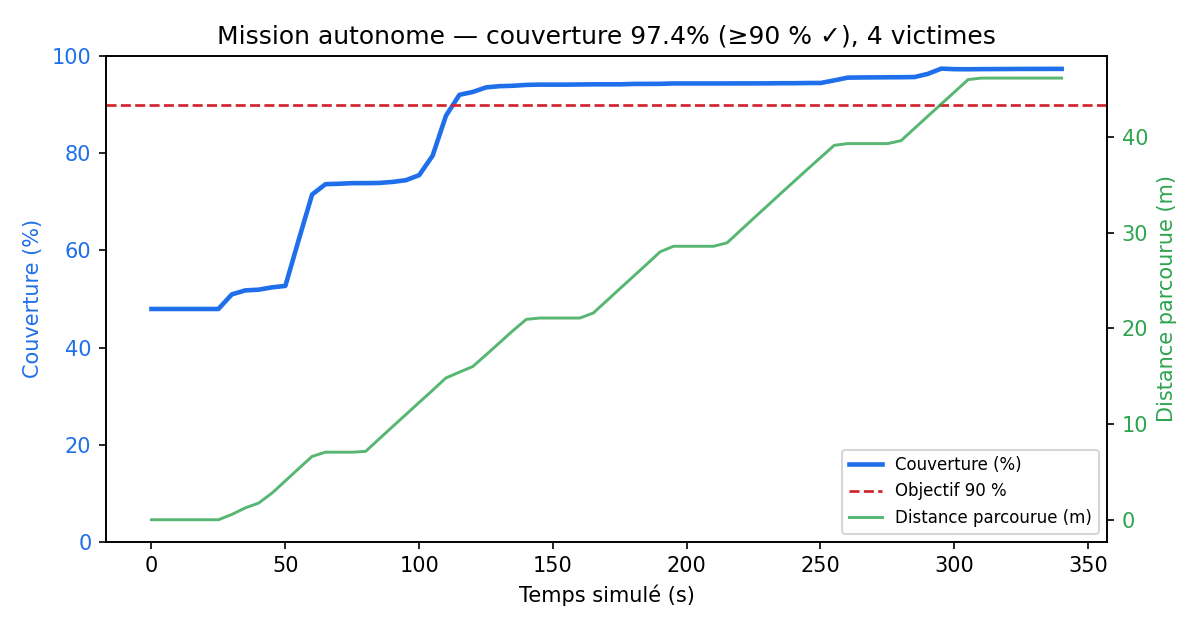
\includegraphics[width=\linewidth]{coverage_curve}\caption{Couverture et longueur de chemin selon le temps, face \`a la cible de 90\,\%.}\end{subfigure}\hfill
\begin{subfigure}{0.44\linewidth}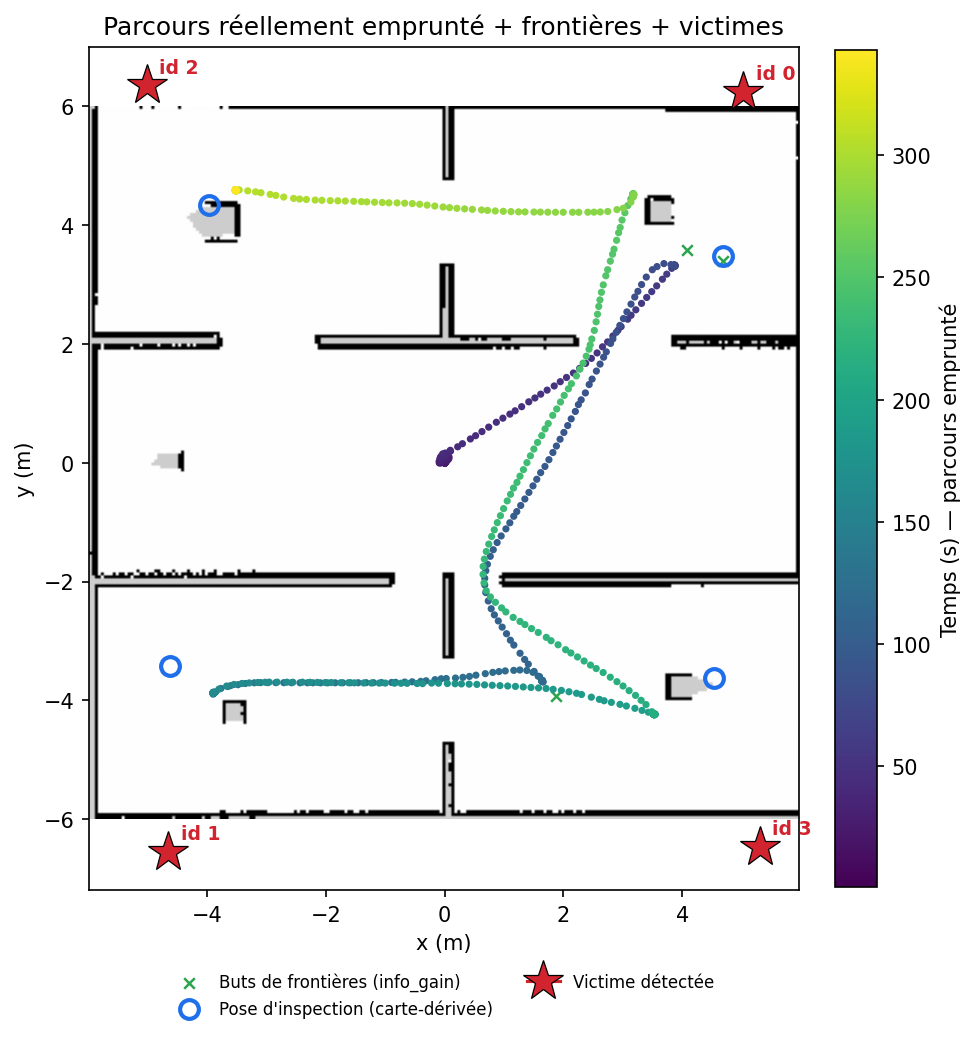
\includegraphics[width=\linewidth]{trajectory_map}\caption{Trajectoire enregistr\'ee (rep\`ere \texttt{map}), color\'ee par le temps, traversant les portes.}\end{subfigure}
\caption{R\'esultats quantitatifs de l'ex\'ecution finale : \textbf{97,35\,\%} de couverture et
\textbf{4/4} victimes, enti\`erement autonome.}
\label{fig:results}
\end{figure}

\begin{figure}[t]
\centering
\begin{subfigure}{0.52\linewidth}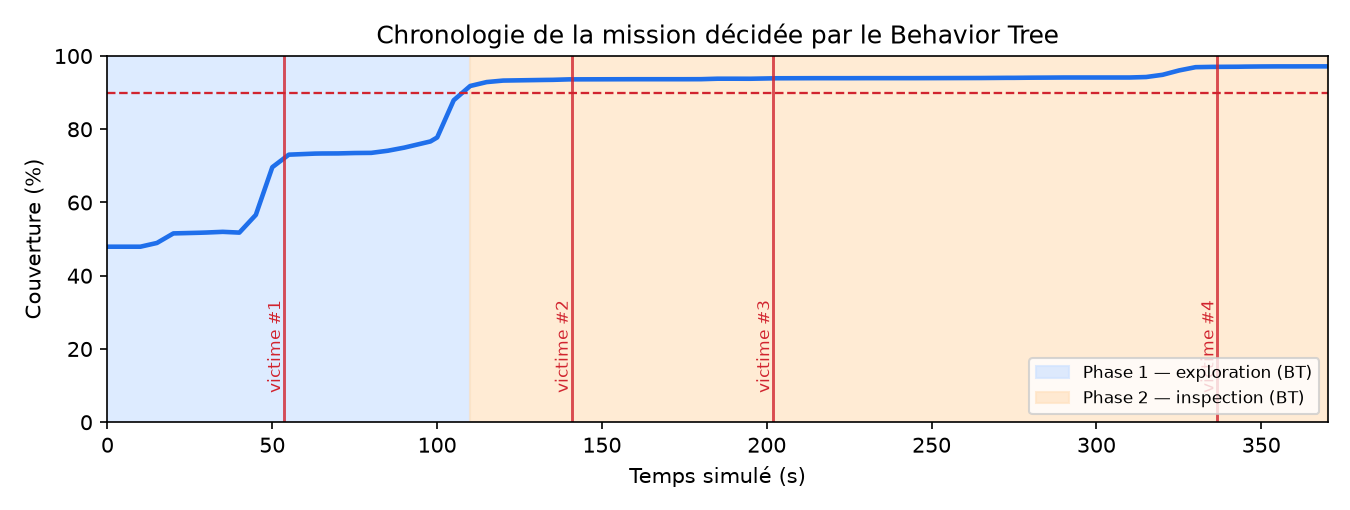
\includegraphics[width=\linewidth]{mission_timeline}\caption{Chronologie d\'ecid\'ee par l'arbre : bandes Phase~1 (bleu) / Phase~2 (orange) et instants de d\'etection.}\end{subfigure}\hfill
\begin{subfigure}{0.29\linewidth}
\includegraphics[width=\linewidth]{mission_map}\caption{Carte finale : quatre victimes et le circuit d'inspection.}\end{subfigure}
\caption{Chronologie de la mission et livrable du sujet : une carte finale annot\'ee de toutes les
positions de victimes.}
\label{fig:timeline}
\end{figure}

\head{Banc d'essai quantitatif d'exploration.} Un banc d'essai bonus ($n{=}3$) confirme la th\'eorie : la
s\'election par gain d'information atteint $0{,}85\pm0{,}08$ de couverture - la seule strat\'egie
au-dessus de la cible de 90\,\% - contre $0{,}72$ pour la s\'election gloutonne. L'avantage vient de
noter les fronti\`eres par le co\^ut de chemin Nav2 plut\^ot que la distance \`a vol d'oiseau, ce qui
\'evite de s'engager vers une fronti\`ere proche mais s\'epar\'ee par un mur.

\head{Parcours d'ing\'enierie.} Atteindre 4/4 ne fut pas imm\'ediat. L'exploration pure donnait une carte
propre mais seulement $\sim$2 victimes et r\'ev\'elait deux causes ind\'ependantes cach\'ees sous le m\^eme
sympt\^ome : la fonction de co\^ut Nav2 d\'ecourageait le robot d'\emph{entrer} dans les pi\`eces (un
probl\`eme de couverture, corrig\'e en abaissant le rayon d'inflation), et un facteur temps-r\'eel
effondr\'e \emph{affamait le rendu de la cam\'era} (un probl\`eme de d\'etection trompeur). Ajouter
l'inspection en deux phases a donn\'e 4/4 et 97\,\% en une ex\'ecution ; nous avons gard\'e un facteur
temps-r\'eel de 0,7, un r\'eglage plus rapide co\^utant une victime et sollicitant trop le GPU.

% 4. CONCLUSION
\section{Conclusion}
Nous avons construit une cha\^ine compl\`ete et conforme au sujet de recherche et sauvetage autonome
autour d'un seul TurtleBot~4 : cartographie par SLAM, exploration par fronti\`eres avec crit\`ere de gain
d'information, projection TF2 des d\'etections AprilTag dans le rep\`ere global, et un arbre de
comportement qui \emph{orchestre} une mission en deux phases. La le\c{c}on cl\'e est que la compl\'etude
de la carte et la couverture des victimes sont des objectifs distincts ; une phase d'inspection autonome
d\'eriv\'ee de la carte les r\'econcilie et fait passer la d\'etection de $\sim$2/4 \`a 4/4 tout en
maintenant 97,35\,\% de couverture. Plus largement, le projet a renforc\'e trois principes :
\emph{mesurer avant de prescrire}, \emph{une correction r\'ev\`ele la suivante} et \emph{le robuste vaut
mieux que le rigide}. Les perspectives incluent l'exploration RRT et un d\'etecteur de victimes appris.

\section*{Remerciements}
Nous remercions chaleureusement \textbf{Zhi Yan}, enseignant-chercheur \`a l'ENSTA, pour le cours IA712 et
l'accompagnement qui ont rendu ce projet possible.

% REFERENCES
\begingroup
\scriptsize
\begin{thebibliography}{9}
\setlength{\itemsep}{0pt}
\setlength{\parskip}{0pt}
\bibitem{assign} IA712 Robotique mobile - Projet final, Projet~B (sujet). \url{https://yzrobot.github.io/IA712/}.
\bibitem{yamauchi} B.~Yamauchi, « A frontier-based approach for autonomous exploration », \emph{IEEE CIRA}, 1997.
\bibitem{slamtb} S.~Macenski, I.~Jambrecic, « slam\_toolbox: SLAM for the dynamic world », \emph{JOSS}, 2021.
\bibitem{nav2} S.~Macenski et al., « The Marathon~2: A navigation system (Nav2) », \emph{IROS}, 2020.
\bibitem{apriltag} E.~Olson, « AprilTag: A robust and flexible visual fiducial system », \emph{ICRA}, 2011.
\end{thebibliography}
\endgroup

\end{document}
